\documentclass[11pt, letterpaper, twoside, openright]{book}

\usepackage{amscd}
\usepackage{amsfonts}
\usepackage{amsmath}
\usepackage{amsrefs}
\usepackage{amssymb}
\usepackage{amsthm}
\usepackage{array}
\usepackage{arydshln}
\usepackage{bbm}
\usepackage{calc}
\usepackage[labelformat=empty, font=bf]{caption}
\usepackage{color}
\usepackage{enumerate}
\usepackage{epsfig}
\usepackage{epstopdf}
\usepackage{etoolbox}
\usepackage{eucal}
\usepackage{fix-cm}
\usepackage{graphicx}
\usepackage{hyperref}
\usepackage{latexsym}
\usepackage{lscape}
\usepackage{mathrsfs}
\usepackage{multicol}
\usepackage{multirow}
\usepackage{pgfplots}
\usepackage{rotating}
\usepackage{setspace}
\usepackage{soul}
\usepackage{stmaryrd}
\usepackage{textcomp}
\usepackage{tikz}
\usepackage{verbatim}
\usepackage{vwcol}
\usepackage[all]{xy}
\usepackage{xparse}
\NewDocumentCommand{\projectchapter}{o m m}{%
\IfNoValueTF{#1}
{\chapter[#2]{#2\origtitle{#3}}}
{\chapter[#1]{#2\origtitle{#3}}}%
}
\newcommand\origtitle[1]{\\
\parbox{\textwidth}{\normalsize\vspace*{2\baselineskip}#1}}
%%%%%%% YOU SHOULDN'T NEED TO ADD ANY PACKAGES. IF YOU DO, PLEASE LET ME KNOW.
\let\TAB\tabular
\renewcommand\tabular{\noindent\TAB}    

\usetikzlibrary{chains,fit,shapes}
\usepackage{ulem}
\tikzstyle{tmtape}=[draw,minimum size=0.7cm]
\tikzstyle{large}=[minimum width=1.5cm]
\tikzstyle{current}=[draw=red!50]
\begin{document}
\mainmatter

\projectchapter{A Game We Can't Win: Undecidability of Quantificational Logic}
{Jonas Wechsler, Mehul Braman, Sam Grayson}

\begin{flushright}
\textit{"I know that I know nothing."} \\
- Socrates
\end{flushright}

General Todos: italicize the first instance of vocabulary words, format graphics better, refer to graphics as fig n, format theorems and defns, spellcheck.

\section{Computers}  %%USE SECTIONS AND SUBSECTIONS TO STRUCTURE YOUR PAPER
\subsection{Alan Turing's life}
%Is ths too similar to wikipedia?
Alan Turing was born on June 23, 1912 in London, while his father was on leave for his position in the Indian Civil Service. His father's civil service was active throughout Turing's childhood, so he and his brother stayed with a retired Army couple whle their parents were traveling. While growing up he attended a day school, St. Michael's, at the age of 6, where his skills in mathematics were well respected by the teachers. At the age of 13, he moved to Sherborne School, a well known independant boys public school. Unfortunately, science and math were not as respected at this school. Once, his headmaster wrote to his parents, "I hope he will not fall between two stools. If he is to stay at public school, he must aim at becoming educated. If he is to be solely a Scientific Specialist, he is wasting his time at a publicschool".

After grade school, Turing studied and subsequently taught mathematics at Cambridge. At Cambridge, he wrote "On Computable Numbers, with an Application to the Entscheidungsproblem", a paper on the limits of proof and computation that created formal and simple hypothetical devices that ultimately became known as Turing Machines.

In 1936, Turing moved to Princeton, though he returned to England in 1938, when he began working for the British cryptanalytic department in a secret part-time job for the Government Code and Cypher School. Following the onset of World War II, he began working full-time at the department's headquarters, Bletchley Park.

==

\subsection{Turing Machines' Formal definition}
A Turing Machine is an idealized kind of computer. Imagine an infinitely long tape divided horizontally into square cells (like movie reel tape). Each cell has a single unit of data written on it. There is a head (something like a box that can read the tape and write on the tape) situated in the middle of the tape (with infinitely many cells to the left, and infinitely many cells to the right) which can move along the tape. This unit moves up and down the tape and, reading and writing to the cells depending on their contents. (TODO: picture).

The head has an internal state or a set of rules that describe how the head operates. Every cycle, it reads the current cell, and based on the state decides what to write to the current cell, and whether to move the tape to the right or move to the left. There is a special state called 'halt' which indicates the machine is done executing the program. (TODO: picture)

A program for the turing machine consists of an alphabet of data that can be written to the tape, a set of states which describe how the head operates, and a tape with default values on it. There is a special symbol for the tape which means `blank' and a spacial state which means `halt' and `crash'. The rest is up to the programmer.

\subsection{Example Turing Program: Search for a character}
Let our alphabet be $\{0, 1, A\}$, where $0$ denotes the blank. Lets say the tape has exactly one $A$ and we want to search to the left until we are at the position of $A$. This function will become useful later.

The following diagram is an example of the tape. The tape extends \textit{ad infinitum} to the left and to the right. The Turing Machine's head is currently over the red cell.

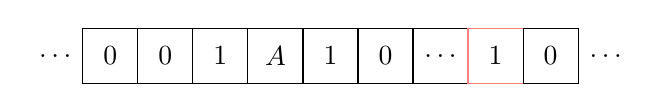
\begin{tikzpicture}
\begin{scope}[start chain=1 going right, node distance=-0.15mm]
    \node [on chain=1,tmtape,draw=none] {$\ldots$};
    \node [on chain=1,tmtape] {0};
    \node [on chain=1,tmtape] {0};
    \node [on chain=1,tmtape] {1};
    \node [on chain=1,tmtape] {$A$};
    \node [on chain=1,tmtape] {1};
    \node [on chain=1,tmtape] {0};
    \node [on chain=1,tmtape] {$\ldots$};
    \node [on chain=1,tmtape,current] {1};
    \node [on chain=1,tmtape] {0};
    \node [on chain=1,tmtape,draw=none] {$\ldots$};
\end{scope}
\end{tikzpicture}

To actually program the Turing Machine, I need to specify states that, given the symbol in the current cell, output what symbol to write, what direction to move, and what next state to go to. I have a `rewind' state, where if the current symbols on the tape is $A$, it halts. Otherwise, it moves left and repeats the process. I also have a `halt' state which indicates the Turing Machine is done executing.

\begin{tabular}{|l|l|l|l|l|l|}
\hline
Current state & Symbol read & Symbol wrote & Movement & Next state \\
\hline
Rewind & $A$ & $A$ & No movement & Halt \\
 & 0 & 0 & Left & Rewind \\
 & 1 & 1 & Left & Rewind \\
\hline
\end{tabular}

This program accomplishes the desired task. It moves one-by-one to the left until it gets to the right cell. Note that recursion is a very useful construct. A state is allowed to execute an action and then repeat. But if a state can repeat itself, there is a chance it will end in an infinite loop. What happens if we start the head

\subsection{Example Turing Program: Incrementing and decrementing}
Given a tape that has a number encoded in binary, I want write a program to increment the number by one. I will start the Turing Machine over the least significant bit, (place value of one). The number will be terminated on the left side by an $A$

In base 10 addition, when you the sum of the digits in a column exceed 10, you let the numbers `wrap around' and then add one to the next higher place value. (TODO: picture). In base 2 addition (binary), this works in a similar way. When you have $1 + 1$ in any column, you set the result to $0$ (since $2$ wraps around to $0$), then add one to the next higher place value, so the result is $10$.

TODO: more example

If that bit is a $0$, to increment it we change it to a $1$. If the bit is a $1$, we set it to $0$ have to carry one. Notice that to carry one, we just add one to the second lowest significant bit (place value of two), move to the left, and increment from that position. If we have to carry so much that we hit the left delimiter $A$, that means the number is too big to fit in the space provided. This is called an integer overflow. I want the program to crash.

\begin{tabular}{|l|l|l|l|l|l|}
\hline
Current state & Symbol read & Symbol wrote & Movement & Next state \\
\hline
Increment & 0 & 1 & No movement & Halt \\
 & 1 & 0 & Left & Increment \\
 & $A$ & $A$ & No movement & Crash (overflow) \\
\hline
\end{tabular}

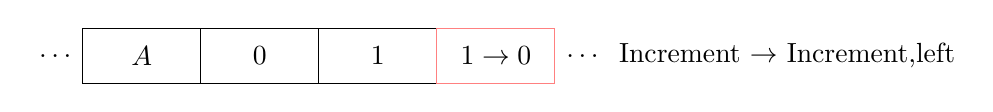
\begin{tikzpicture}
\begin{scope}[start chain=1 going right, node distance=-0.15mm]
    \node [on chain=1,tmtape,draw=none] {$\ldots$};
    \node [on chain=1,tmtape,large] {$A$};
    \node [on chain=1,tmtape,large] {0};
    \node [on chain=1,tmtape,large] {1};
    \node [on chain=1,tmtape,large,current] {$1 \to 0$};
    \node [on chain=1,tmtape,draw=none] {$\ldots$};
    \node [on chain=1] {Increment $\to$ Increment,\break left};
\end{scope}
\end{tikzpicture}

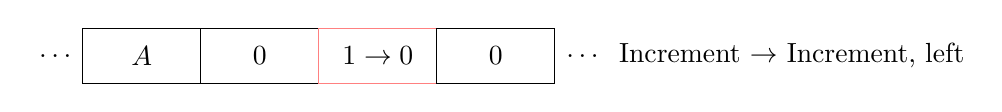
\begin{tikzpicture}
\begin{scope}[start chain=1 going right, node distance=-0.15mm]
    \node [on chain=1,tmtape,draw=none] {$\ldots$};
    \node [on chain=1,tmtape,large] {$A$};
    \node [on chain=1,tmtape,large] {0};
    \node [on chain=1,tmtape,large,current] {$1 \to 0$};
    \node [on chain=1,tmtape,large] {0};
    \node [on chain=1,tmtape,draw=none] {$\ldots$};
    \node [on chain=1] {Increment $\to$ Increment, left};
\end{scope}
\end{tikzpicture}

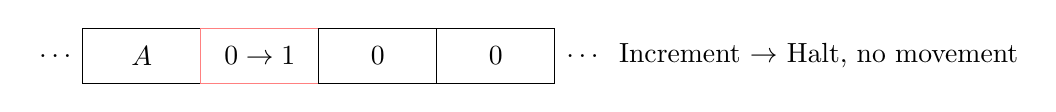
\begin{tikzpicture}
\begin{scope}[start chain=1 going right, node distance=-0.15mm]
    \node [on chain=1,tmtape,draw=none] {$\ldots$};
    \node [on chain=1,tmtape,large] {$A$};
    \node [on chain=1,tmtape,large,current] {$0 \to 1$};
    \node [on chain=1,tmtape,large] {0};
    \node [on chain=1,tmtape,large] {0};
    \node [on chain=1,tmtape,draw=none] {$\ldots$};
    \node [on chain=1] {Increment $\to$ Halt, no movement};
\end{scope}
\end{tikzpicture}

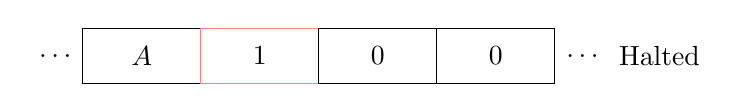
\begin{tikzpicture}
\begin{scope}[start chain=1 going right, node distance=-0.15mm]
    \node [on chain=1,tmtape,draw=none] {$\ldots$};
    \node [on chain=1,tmtape,large] {$A$};
    \node [on chain=1,tmtape,large,current] {1};
    \node [on chain=1,tmtape,large] {0};
    \node [on chain=1,tmtape,large] {0};
    \node [on chain=1,tmtape,draw=none] {$\ldots$};
    \node [on chain=1] {Halted};
\end{scope}
\end{tikzpicture}

The tape below is set up to increment 3 (011). It adds one getting 4 (100), carrying twice. Decrementing works the same way, except the $1$ and $0$ are switched, so 0 $\to$ 1, decrement $\to$ decrement (carry one), and 1 $\to$ 0,
decrement $\to$ halt.

\begin{tabular}{|l|l|l|l|l|l|}
\hline
Current state & Symbol read & Symbol wrote & Movement & Next state \\
\hline
Decrement & 1 & 0 & No movement & Halt \\
 & 0 & 1 & Left & Increment \\
 & $A$ & $A$ & No movement & Crash (underflow) \\
\hline
\end{tabular}

Not that when we try to decrement from the tape $A0000$, we find $0$ as the current symbol, change it to $1$, move to the left, and repeat (carry one). Then we find $0$ as the current symbol, change it to a $1$, move to the left, and repeat until we reach $A$ which tells us that the integer underflowed.

\subsection{Example Turing Program: Adding Natural Numbers}
Let our alphabet be the ${0, 1, A, B, C, D}$, where $0$ denotes a blank. We want to put the first number on the tape towards the left, and then the second number towards the right. In order for the Turing Machine to know where the numbers start and end, I will put an $A$ to denote the start of the first number, $B$ for its end, $C$ for the start of the second number, and $D$ for its end. Let the turing machine start anywhere to the right of $B$.

The following diagram is an example of the tap for this program set to compute 5 + 6. The 5 is between $A$ and $B$. The 6 is between $C$ and $D$. There can be an arbitrary amount of data between $B$ and $C$; It is all ignored by the program. This will become important later.

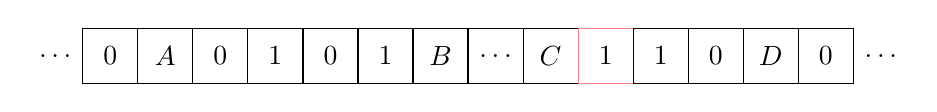
\begin{tikzpicture}
\begin{scope}[start chain=1 going right, node distance=-0.15mm]
    \node [on chain=1,tmtape,draw=none] {$\ldots$};
    \node [on chain=1,tmtape] {0};
    \node [on chain=1,tmtape] {$A$};
    \node [on chain=1,tmtape] {0};
    \node [on chain=1,tmtape] {1};
    \node [on chain=1,tmtape] {0};
    \node [on chain=1,tmtape] {1};
    \node [on chain=1,tmtape] {$B$};
    \node [on chain=1,tmtape] {$\ldots$};
    \node [on chain=1,tmtape] {$C$};
    \node [on chain=1,tmtape,current] {1};
    \node [on chain=1,tmtape] {1};
    \node [on chain=1,tmtape] {0};
    \node [on chain=1,tmtape] {$D$};
    \node [on chain=1,tmtape] {0};
    \node [on chain=1,tmtape,draw=none] {$\ldots$};
\end{scope}
\end{tikzpicture}

In general want to decrement the first number and increment the second number until the first number is zero. Then we know the sum is stored where the second number used to be second number (between $C$ and $D$).

\begin{enumerate}
\item In the style of the first example, I will navigate to the start of the first number (denoted by $B$) using the state `rewind'. This state moves to the left until it hits a $B$, and then moves exactly once more to the left.

\item Using the second example, I will decrement the first number by one under the state `decrement'. If the there is an underflow, that means I tried to decrement from zero, therefore the machine is done adding and it should halt.

\item Otherwise I want the machine to move back to the start of the second number (deonted by $D$) under state `forward'.

\item Now that the head is positioned, I want to increment the second number by one using the `increment' state. If there is an integer overflow, the second block of memory is not large enough to store the result, so the machine crashes. Otherwise repeat.
\end{enumerate}

\begin{tabular}{|l|l|l|l|l|l|}
\hline
Current state & Symbol read & Symbol wrote & Movement & Next state \\
\hline
Rewind & B & B & Left & Decrement \\
 & \textit{Otherwise} & \textit{None} & Left & Rewind \\
\hline
Decrement & 1 & 0 & Right & Forward \\
 & 0 & 1 & Left & Decrement \\
 & A & A & None & Halt \\
\hline
Forward & D & D & Right & Increment \\
 & \textit{Otherwise} & \textit{None} & Right & Forward \\
\hline
Increment & 0 & 1 & Left & Rewind \\
 & 1 & 0 & Left & Increment \\
 & C & C & None & Crash \\
\hline
\end{tabular}

TODO: show simulation

\subsection{Example Turing Program: Multiplying Natural Numbers}
TODO: adding numbers, save result

TODO: multiply numbers.

\subsection{Example Turing Program: Computing Natural exponents}

\subsection{The Halting Problem}
How can we be sure if a program stops? There is no way to do this!

\section{Axiomatic systems}
\subsection{What is an axiomatic system?}
% The most common way of specifying an interpretation (especially in mathematics) is to specify a structure (also called a model; see below)

You should remember first-order logic has names (also called constants) denoted by lower case letters $a, b, c$, predicates denoted as $Pxy$ or $P(x,y)$ (where the predicate $P$ is acting over the arguments $x$ and $y$), and logical connectives like $\wedge$.

An axiomatic system is a set of sentences in quantificational logic that describe something. These are very useful in mathematics. Natural numbers can be defined as an axiomatic system.

\subsection{Example Axiomatic System: Natural Numbers}
Let $Nx$ mean $x$ is a natural number, and $Sx$ mean the next number after $x$ (also called successor of $x$).
\begin{enumerate}
\item $\neg \exists x (Sx = 0)$ There is not a number whose successor is zero.
\item $\forall x \forall y (Sx = Sy \rightarrow x = y)$ Equal successors ($Sx = Sy$) mean equal numbers $x = y$.
\item $\forall y (\neg y = 0 \rightarrow (\exists x Sx = y))$ Except for zero, every number $y$ is the successor of some number $x$.
\item $\forall x (x + 0 = x)$ Identity property of addition.
\item $\forall x \forall y (x + S(y) = S(x + y))$ Defines addition recursively (together with the identity property)
\item $\forall x (x \cdot 0 = 0)$ Zero property of multiplication
\item $\forall x \forall y (x \cdot Sy = x \cdot y + x)$ Defines multiplication recursively (together with the identity property)
\item $(P(0) \wedge \forall k (P(k) \rightarrow P(k + 1))) \rightarrow \forall n P(n)$ A statement of induction
\end{enumerate}

This is called \textit{Peano Arithmetic}. There are many different versions, here is a common one. It encodes natural numbers in first-order logic.

\subsection{Models}
You should also remember that we can specify an \textit{interpretation} which is just an example of objects that satisfy make all of the sentences true. We specified models by creating a \textit{model}, which states the universe of discourse and specifying when predicates are true.

\subsection{Consistency}
This is what consistency means.

This is how to prove consistency.

This is how to prove inconsistency.

\subsection{Entscheidungsproblem}
Its really fun to say.

\section{Observations}
\subsection{Church-Turing Hypothesis}
Do you remember the Turing machine? Do you remember axiomatic systems? What if I told you they are the same thing. Any expression that can be evaluated through the use of an axiomatic system can be evaluated through a turing machine. TODO: this

\subsection{G\"{o}del's Incompleteness Theorems}
\textbf{G\"{o}del's First Incompletness Theorem} Every set of axioms is either inconsistent or incomplete, where incomplete means that it cannot prove all truths about the natural numbers.

\textbf{G\"{o}del's Second Incompletness Theorem} The second incompleteness theorem shows that such a system cannot demonstrate its own consistency.

\subsection{Incompleteness implications: ENtscheidungsproblem}
There is no way to perfectly prove things in First-order logic. There are things that are true which we cannot prove.

\subsection{Incompleteness implications: Halting problem}
We can't be sure that a given turing program will halt.

\subsection{Incompletness implications: Continued implications}
You can't prove \textit{everything}. There will always things that are true which you can not prove.

Mathematics is fundamentally \sout{flawed} complicated.

Some people say the universe is fundamentally mathematical. If this is true, then the following syllogism must hold.
\begin{enumerate}
\item All non-trivial computational systems are incomplete
\item The universe is a non-trivial computational system
\item herefore the universe is incomplete
\end{enumerate}

A\`{ }theory of everything''--whether in math, or physics, or philosophy--will never be found. Because it is impossible.

TODO: this

\end{document}

%%% Local Variables: 
%%% mode: latex 
%%% TeX-master: t 
%%% End:
